\documentclass[12pt,journal]{IEEEtran}

\usepackage[utf8]{inputenc}
\usepackage{pgfplots}
\usepackage{caption}

\begin{document}

    \title{Derivative fundamentals}
    \author{Alejandro Salgado Gomez}

    \maketitle

    This article will try to explain as simple as posible the concept of a
    derivative. A derivatavie is the solution to one of the principal
    problems in calculus, which is how to calculate the tangent rect throught
    a point, in other words, how to calculate the rate of change of a function.

    This has a lot of practical applications in mathematics and the real
    world\\

    Lets start from the beginning, lets say we have two points that represent
    the state of something that is moving, the first one is the starting
    position and the second one is the position after a slide of time. And we
    want to calculate how much is the change of the possition of this thing
    from the starting point to the final position. Here a ilustration\\

    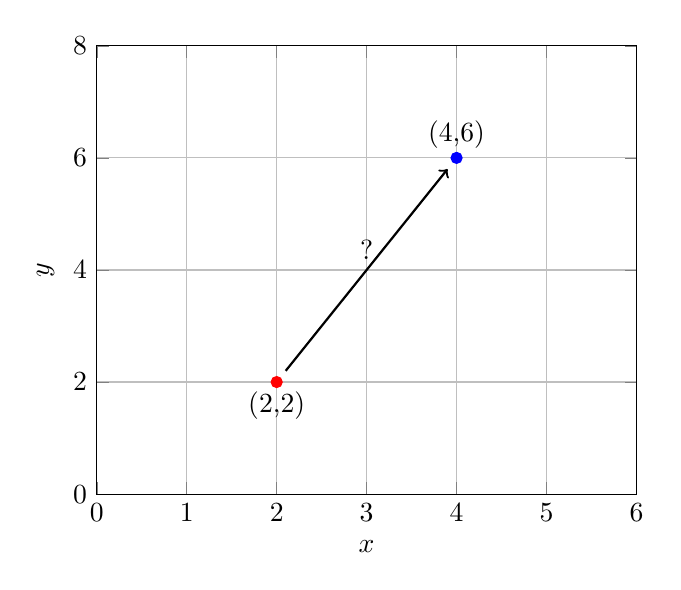
\begin{tikzpicture}
        \begin{axis}[
                      xlabel=$x$,
                      ylabel=$y$,
                      xmin=0, xmax=6,
                      ymin=0, ymax=8,
                      grid=both
                    ]
            \addplot[color=red, only marks]
                coordinates{
                    (2,2)
                };

            \node[below] at (axis cs: 2,2) {(2,2)};

            \addplot[color=blue, only marks]
                coordinates{
                    (4,6)
                };

            \node[above] at (axis cs: 4,6) {(4,6)};

            \draw[thick,->] (axis cs: 2.1,2.2) -- node[above]{?} (axis cs: 3.9,5.8);
        \end{axis}
    \end{tikzpicture}

    Notice that we are not interested in calculate the distance between this
    points, what we want to find is a number that decribes how much the thing's
    position has change when he moves from the beginning to the second possition.

    This can be done by calculating for each unit of distance that the object
    has move, how much the object assend. This calculus can be  described as
    follows

    \begin{equation}
        change = \frac{ascend}{advance}
    \end{equation}

    \vspace{1cm}

    For the example the formula would be $change = \frac{2}{1} = 2$, this
    means that every time that the thing moves 1 unit, also assend two units.
    Now the illustration \\

    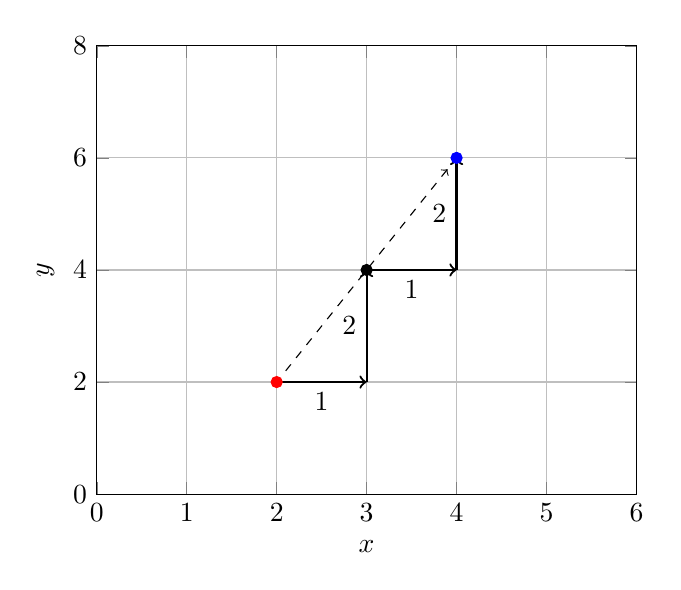
\begin{tikzpicture}
        \begin{axis}[
                      xlabel=$x$,
                      ylabel=$y$,
                      xmin=0, xmax=6,
                      ymin=0, ymax=8,
                      grid=both
                    ]
            \addplot[color=red, only marks]
                coordinates{
                    (2,2)
                };

            \addplot[color=black, only marks]
                coordinates{
                    (3,4)
                };

            \addplot[color=blue, only marks]
                coordinates{
                    (4,6)
                };

            \draw[dashed,->] (axis cs: 2.1,2.2) -- (axis cs: 3.9,5.8);

            \draw[thick,->] (axis cs: 2,2) -- node[below]{1} (axis cs: 3,2);
            \draw[thick,->] (axis cs: 3,2) -- node[left]{2} (axis cs: 3,4);

            \draw[thick,->] (axis cs: 3,4) -- node[below]{1} (axis cs: 4,4);
            \draw[thick,->] (axis cs: 4,4) -- node[left]{2} (axis cs: 4,6);
        \end{axis}
    \end{tikzpicture}

    Now that we know the "rate of change" of the movement we can calculate which
    would be the position of the object at any moment of the movement, this means
    that we can know the position when the object has move 1 unit, 2 units, or
    any amount of units that we want.

    \begin{figure}[h]
        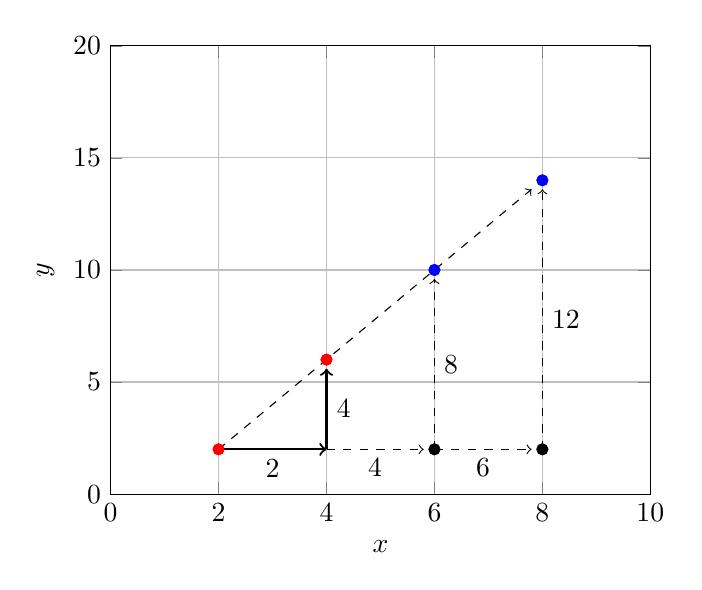
\begin{tikzpicture}
            \begin{axis}[
                          xlabel=$x$,
                          ylabel=$y$,
                          xmin=0, xmax=10,
                          ymin=0, ymax=20,
                          grid=both
                        ]
                \addplot[color=red, only marks]
                    coordinates{
                        (2,2)
                        (4,6)
                    };

                \addplot[color=blue, only marks]
                    coordinates{
                        (6,10)
                        (8,14)
                    };

                \addplot[color=black, only marks]
                    coordinates{
                        (6,2)
                        (8,2)
                    };

                \draw[thick,->] (axis cs: 2,2) -- node[below]{2} (axis cs: 4,2);
                \draw[thick,->] (axis cs: 4,2) -- node[right]{4} (axis cs: 4,5.6);

                \draw[dashed,->] (axis cs: 4,2) -- node[below]{4} (axis cs: 5.8,2);
                \draw[dashed,->] (axis cs: 6,2) -- node[right]{8} (axis cs: 6,9.6);

                \draw[dashed,->] (axis cs: 6,2) -- node[below]{6} (axis cs: 7.8,2);
                \draw[dashed,->] (axis cs: 8,2) -- node[right]{12} (axis cs: 8,13.6);

                \draw[dashed,->] (axis cs: 2,2) -- (axis cs: 7.8,13.6);
            \end{axis}
        \end{tikzpicture}
    \end{figure}

    This means that now we can predict how is going to be the movement of the
    object. All we have to do is take the units of movement that we want in the
    horizontal axis and then multiply that number for the change that we found
    before and thats all.\\

    Now we are going to formalize this concept a little bit. First we are going
    to change the name of the variable "change" to just a letter for simplicity,
    lets say "m". \\

    $change = m$ \\

    Now we are going to take the define the horizontal distance between the points
    as the difference between the two $x$ components and the vertical distance as
    the difference between the two $y$ components. In mathematics the difference
    between a same variable is denoted as $\Delta$variable, this means that the
    difference between the $x$ component will be $\Delta x$ and the difference
    between the $y$ components will be $\Delta y$\\

    \begin{tikzpicture}
        \begin{axis}[
                      xlabel=$x$,
                      ylabel=$y$,
                      xmin=0, xmax=7,
                      ymin=0, ymax=8,
                      xtick=\empty,
                      ytick=\empty,
                    ]
            \addplot[color=red, only marks]
                coordinates{
                    (2,2)
                };
            \node[above] at (axis cs: 2,2) {($x_1$,$y_1$)};

            \addplot[color=blue, only marks]
                coordinates{
                    (4,6)
                };
            \node[left] at (axis cs: 4,6) {($x_2$,$y_2$)};

            \draw[thick] (axis cs: 2,2) -- node[below]{$x_1 - x_2 = \Delta x$}(axis cs: 4,2);
            \draw[thick] (axis cs: 4,2) -- node[right]{$y_1 - y_2 = \Delta y$} (axis cs: 4,6);
        \end{axis}
    \end{tikzpicture}

    Then we can define the change as follows

    \begin{equation}
        m = \frac{\Delta y}{\Delta x}
    \end{equation}

    The last formula is the formal definition of the slope in mathematics, this
    is the change of state in a point of a linear function, just like we have
    explained earlier.

    This works very good for any linear function, but what happens when we
    whant to analise a non linear function like a curve?. Lets see an example

    \begin{tikzpicture}
        \begin{axis}[
                      xlabel=$x$,
                      ylabel=$y$,
                      xmin=0, xmax=6,
                      ytick=\empty
                    ]

            \addplot[color=blue]{x^4};

            \addplot[color=red, only marks]
                coordinates{
                    (1,1)
                };

            \addplot[color=red, only marks]
                coordinates{
                    (4.8,530)
                };

            \addplot[color=black]{139.2*x -138.2};
        \end{axis}
    \end{tikzpicture}

\end{document}
